\documentclass[twoside]{book}

% Packages required by doxygen
\usepackage{fixltx2e}
\usepackage{calc}
\usepackage{doxygen}
\usepackage[export]{adjustbox} % also loads graphicx
\usepackage{graphicx}
\usepackage[utf8]{inputenc}
\usepackage{makeidx}
\usepackage{multicol}
\usepackage{multirow}
\PassOptionsToPackage{warn}{textcomp}
\usepackage{textcomp}
\usepackage[nointegrals]{wasysym}
\usepackage[table]{xcolor}

% Font selection
\usepackage[T1]{fontenc}
\usepackage[scaled=.90]{helvet}
\usepackage{courier}
\usepackage{amssymb}
\usepackage{sectsty}
\renewcommand{\familydefault}{\sfdefault}
\allsectionsfont{%
  \fontseries{bc}\selectfont%
  \color{darkgray}%
}
\renewcommand{\DoxyLabelFont}{%
  \fontseries{bc}\selectfont%
  \color{darkgray}%
}
\newcommand{\+}{\discretionary{\mbox{\scriptsize$\hookleftarrow$}}{}{}}

% Page & text layout
\usepackage{geometry}
\geometry{%
  a4paper,%
  top=2.5cm,%
  bottom=2.5cm,%
  left=2.5cm,%
  right=2.5cm%
}
\tolerance=750
\hfuzz=15pt
\hbadness=750
\setlength{\emergencystretch}{15pt}
\setlength{\parindent}{0cm}
\setlength{\parskip}{3ex plus 2ex minus 2ex}
\makeatletter
\renewcommand{\paragraph}{%
  \@startsection{paragraph}{4}{0ex}{-1.0ex}{1.0ex}{%
    \normalfont\normalsize\bfseries\SS@parafont%
  }%
}
\renewcommand{\subparagraph}{%
  \@startsection{subparagraph}{5}{0ex}{-1.0ex}{1.0ex}{%
    \normalfont\normalsize\bfseries\SS@subparafont%
  }%
}
\makeatother

% Headers & footers
\usepackage{fancyhdr}
\pagestyle{fancyplain}
\fancyhead[LE]{\fancyplain{}{\bfseries\thepage}}
\fancyhead[CE]{\fancyplain{}{}}
\fancyhead[RE]{\fancyplain{}{\bfseries\leftmark}}
\fancyhead[LO]{\fancyplain{}{\bfseries\rightmark}}
\fancyhead[CO]{\fancyplain{}{}}
\fancyhead[RO]{\fancyplain{}{\bfseries\thepage}}
\fancyfoot[LE]{\fancyplain{}{}}
\fancyfoot[CE]{\fancyplain{}{}}
\fancyfoot[RE]{\fancyplain{}{\bfseries\scriptsize Generated by Doxygen }}
\fancyfoot[LO]{\fancyplain{}{\bfseries\scriptsize Generated by Doxygen }}
\fancyfoot[CO]{\fancyplain{}{}}
\fancyfoot[RO]{\fancyplain{}{}}
\renewcommand{\footrulewidth}{0.4pt}
\renewcommand{\chaptermark}[1]{%
  \markboth{#1}{}%
}
\renewcommand{\sectionmark}[1]{%
  \markright{\thesection\ #1}%
}

% Indices & bibliography
\usepackage{natbib}
\usepackage[titles]{tocloft}
\setcounter{tocdepth}{3}
\setcounter{secnumdepth}{5}
\makeindex

% Hyperlinks (required, but should be loaded last)
\usepackage{ifpdf}
\ifpdf
  \usepackage[pdftex,pagebackref=true]{hyperref}
\else
  \usepackage[ps2pdf,pagebackref=true]{hyperref}
\fi
\hypersetup{%
  colorlinks=true,%
  linkcolor=blue,%
  citecolor=blue,%
  unicode%
}

% Custom commands
\newcommand{\clearemptydoublepage}{%
  \newpage{\pagestyle{empty}\cleardoublepage}%
}

\usepackage{caption}
\captionsetup{labelsep=space,justification=centering,font={bf},singlelinecheck=off,skip=4pt,position=top}

%===== C O N T E N T S =====

\begin{document}

% Titlepage & ToC
\hypersetup{pageanchor=false,
             bookmarksnumbered=true,
             pdfencoding=unicode
            }
\pagenumbering{alph}
\begin{titlepage}
\vspace*{7cm}
\begin{center}%
{\Large Reference Manual}\\
\vspace*{1cm}
{\large Generated by Doxygen 1.8.14}\\
\end{center}
\end{titlepage}
\clearemptydoublepage
\pagenumbering{roman}
\tableofcontents
\clearemptydoublepage
\pagenumbering{arabic}
\hypersetup{pageanchor=true}

%--- Begin generated contents ---
\chapter{Sudoku\+Solver}
\label{index}\hypertarget{index}{}Simple Sudoku puzzle solver built in Qt. 
\chapter{Hierarchical Index}
\section{Class Hierarchy}
This inheritance list is sorted roughly, but not completely, alphabetically\+:\begin{DoxyCompactList}
\item Q\+Object\begin{DoxyCompactList}
\item \contentsline{section}{Solver\+Engine}{\pageref{class_solver_engine}}{}
\end{DoxyCompactList}
\item \contentsline{section}{Solver\+Engine\+:\+:x\+Location\+\_\+t}{\pageref{struct_solver_engine_1_1x_location__t}}{}
\end{DoxyCompactList}

\chapter{Class Index}
\section{Class List}
Here are the classes, structs, unions and interfaces with brief descriptions\+:\begin{DoxyCompactList}
\item\contentsline{section}{\mbox{\hyperlink{class_solver_engine}{Solver\+Engine}} \\*Class containing all functionality required for modeling, solving, and managing puzzles }{\pageref{class_solver_engine}}{}
\item\contentsline{section}{\mbox{\hyperlink{struct_solver_engine_1_1x_location__t}{Solver\+Engine\+::x\+Location\+\_\+t}} \\*Struct for holding a location on the board, consisting of a row and column position }{\pageref{struct_solver_engine_1_1x_location__t}}{}
\end{DoxyCompactList}

\chapter{File Index}
\section{File List}
Here is a list of all files with brief descriptions\+:\begin{DoxyCompactList}
\item\contentsline{section}{src/\mbox{\hyperlink{main_8cpp}{main.\+cpp}} \\*Source file containing the main entry point for the application }{\pageref{main_8cpp}}{}
\item\contentsline{section}{src/\mbox{\hyperlink{solverengine_8cpp}{solverengine.\+cpp}} \\*Source file for the engine class }{\pageref{solverengine_8cpp}}{}
\item\contentsline{section}{src/\mbox{\hyperlink{solverengine_8h}{solverengine.\+h}} \\*Contains the functionality for the engine used to model and solve puzzles as well as controlling the view }{\pageref{solverengine_8h}}{}
\end{DoxyCompactList}

\chapter{Class Documentation}
\hypertarget{class_solver_engine}{}\section{Solver\+Engine Class Reference}
\label{class_solver_engine}\index{Solver\+Engine@{Solver\+Engine}}


Class containing all functionality required for modeling, solving, and managing puzzles.  




{\ttfamily \#include $<$solverengine.\+h$>$}

Inheritance diagram for Solver\+Engine\+:\begin{figure}[H]
\begin{center}
\leavevmode
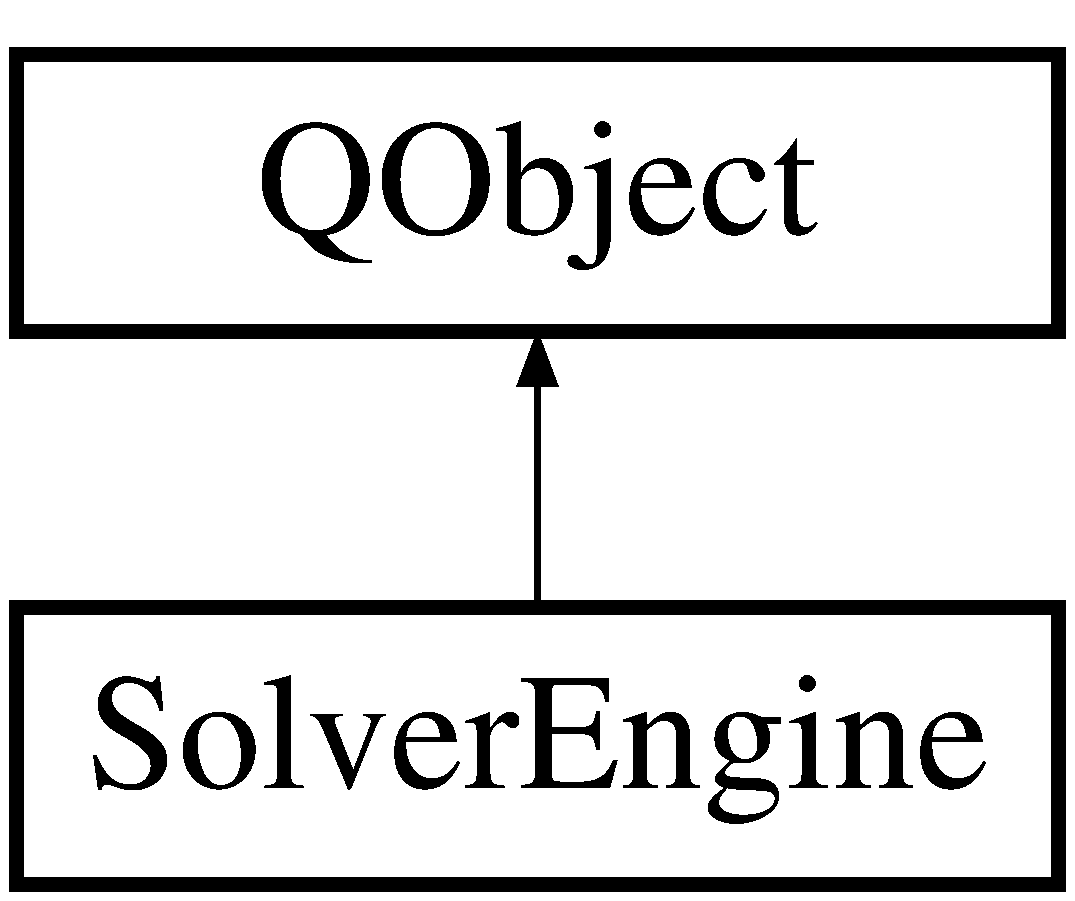
\includegraphics[height=2.000000cm]{class_solver_engine}
\end{center}
\end{figure}
\subsection*{Classes}
\begin{DoxyCompactItemize}
\item 
struct \mbox{\hyperlink{struct_solver_engine_1_1x_location__t}{x\+Location\+\_\+t}}
\begin{DoxyCompactList}\small\item\em Struct for holding a location on the board, consisting of a row and column position. \end{DoxyCompactList}\end{DoxyCompactItemize}
\subsection*{Public Types}
\begin{DoxyCompactItemize}
\item 
enum \mbox{\hyperlink{class_solver_engine_acd25f3521e492d4aa924f922396bf02c}{e\+Engine\+State\+\_\+t}} \{ \mbox{\hyperlink{class_solver_engine_acd25f3521e492d4aa924f922396bf02ca5a2e2dc92b4d1e18ad4143fc1482653c}{Engine\+State\+\_\+\+Idle}} = 0, 
\mbox{\hyperlink{class_solver_engine_acd25f3521e492d4aa924f922396bf02ca75636af1a8b5276f1e7545f6ebb0fd94}{Engine\+State\+\_\+\+Solving}}, 
\mbox{\hyperlink{class_solver_engine_acd25f3521e492d4aa924f922396bf02ca406c53dc180a55ca68b29bd0ca9cd2ed}{Engine\+State\+\_\+\+Finished}}, 
\mbox{\hyperlink{class_solver_engine_acd25f3521e492d4aa924f922396bf02cacb5e7043b14126f8a641f9ec98a481f6}{Engine\+State\+\_\+\+Error}}
 \}
\begin{DoxyCompactList}\small\item\em Enum containing all possible states for the engine, accessible via Q\+ML. \end{DoxyCompactList}\end{DoxyCompactItemize}
\subsection*{Public Slots}
\begin{DoxyCompactItemize}
\item 
void \mbox{\hyperlink{class_solver_engine_a819bfa5cf96fc7fe05e9f091bf2666e2}{solve}} ()
\begin{DoxyCompactList}\small\item\em Commands the engine to start attempting a solution using the current state of the view. \end{DoxyCompactList}\item 
void \mbox{\hyperlink{class_solver_engine_af8e6ec12a994e8a463f2b3b1a0368e33}{reset}} ()
\begin{DoxyCompactList}\small\item\em Clears any currently-\/loaded board and conflicts models. \end{DoxyCompactList}\end{DoxyCompactItemize}
\subsection*{Signals}
\begin{DoxyCompactItemize}
\item 
void \mbox{\hyperlink{class_solver_engine_a73fd20671c169def4c85c53a2102e920}{state\+Changed}} ()
\begin{DoxyCompactList}\small\item\em Signal emitted whenever the engine state changes. \end{DoxyCompactList}\item 
void \mbox{\hyperlink{class_solver_engine_a66c3ab757c4e8aa50484f992f2b1ba7e}{solve\+Time\+Changed}} ()
\begin{DoxyCompactList}\small\item\em Signal emitted whenever the time taken to solve the puzzle is announced. \end{DoxyCompactList}\end{DoxyCompactItemize}
\subsection*{Public Member Functions}
\begin{DoxyCompactItemize}
\item 
\mbox{\hyperlink{class_solver_engine_acd25f3521e492d4aa924f922396bf02c}{e\+Engine\+State\+\_\+t}} \mbox{\hyperlink{class_solver_engine_a74305814124ef4b1ff74b082b53d155c}{state}} () const
\begin{DoxyCompactList}\small\item\em Getter function for the current state of the engine. \end{DoxyCompactList}\item 
double \mbox{\hyperlink{class_solver_engine_af647e59feb82e7a8aa445e1e03a386aa}{solve\+Time}} () const
\begin{DoxyCompactList}\small\item\em Getter function for the time taken by the engine to solve the puzzle once completed. \end{DoxyCompactList}\end{DoxyCompactItemize}
\subsection*{Static Public Member Functions}
\begin{DoxyCompactItemize}
\item 
static \mbox{\hyperlink{class_solver_engine}{Solver\+Engine}} $\ast$ \mbox{\hyperlink{class_solver_engine_abc1e088d35a6702a58c57e3344348eab}{instance}} ()
\begin{DoxyCompactList}\small\item\em Returns the Singleton instance associated with this engine. \end{DoxyCompactList}\end{DoxyCompactItemize}
\subsection*{Properties}
\begin{DoxyCompactItemize}
\item 
int \mbox{\hyperlink{class_solver_engine_a6ac564f91cd5c523ece2c561a37b8263}{state}}
\begin{DoxyCompactList}\small\item\em The current state of the engine. \end{DoxyCompactList}\item 
double \mbox{\hyperlink{class_solver_engine_aac9c7fba1a049fe08bcfd341700840fb}{solve\+Time}}
\begin{DoxyCompactList}\small\item\em The time taken by the engine to solve the last puzzle in seconds. \end{DoxyCompactList}\end{DoxyCompactItemize}
\subsection*{Private Member Functions}
\begin{DoxyCompactItemize}
\item 
\mbox{\hyperlink{class_solver_engine_a677b5fe26a9eea0dea994cc3f9027211}{Solver\+Engine}} ()
\begin{DoxyCompactList}\small\item\em Constructor for the engine, responsible for initializing classing members. \end{DoxyCompactList}\item 
void \mbox{\hyperlink{class_solver_engine_a24a236b02f997c594c259d15167e32d1}{update\+Screen}} ()
\begin{DoxyCompactList}\small\item\em Writes out the current internal board model to the Q\+ML view to display it to the user. \end{DoxyCompactList}\item 
bool \mbox{\hyperlink{class_solver_engine_a8c1f32f617ef8c5b83c4bef56e7dc89a}{solve\+Board}} ()
\begin{DoxyCompactList}\small\item\em Core function for solving the puzzle using the currently-\/loaded internal board model. \end{DoxyCompactList}\item 
\mbox{\hyperlink{struct_solver_engine_1_1x_location__t}{x\+Location\+\_\+t}} \mbox{\hyperlink{class_solver_engine_a27aa053eb5e2a7abb602b7763ec6dea8}{next\+Blank\+Cell}} (const \mbox{\hyperlink{struct_solver_engine_1_1x_location__t}{x\+Location\+\_\+t}} \&x\+Start\+Location=\mbox{\hyperlink{struct_solver_engine_1_1x_location__t}{x\+Location\+\_\+t}}(0, 0)) const
\begin{DoxyCompactList}\small\item\em Finds the next blank cell that is a candidate for value insertion. \end{DoxyCompactList}\item 
bool \mbox{\hyperlink{class_solver_engine_a7e9939f155549012b8be1bb854eba5c3}{can\+Place\+Value}} (const \mbox{\hyperlink{struct_solver_engine_1_1x_location__t}{x\+Location\+\_\+t}} \&x\+Location, int i\+Value) const
\begin{DoxyCompactList}\small\item\em Consults the current conflicts, returning whether or not the proposed value placement is acceptable. \end{DoxyCompactList}\item 
int \mbox{\hyperlink{class_solver_engine_a3b515701f25827a9d817e7ca529f9b80}{square\+Number\+From\+Location}} (const \mbox{\hyperlink{struct_solver_engine_1_1x_location__t}{x\+Location\+\_\+t}} \&x\+Location) const
\begin{DoxyCompactList}\small\item\em Returns the square number containing the passed location on the board. \end{DoxyCompactList}\end{DoxyCompactItemize}
\subsection*{Private Attributes}
\begin{DoxyCompactItemize}
\item 
Q\+Vector$<$ Q\+Vector$<$ int $>$ $>$ \mbox{\hyperlink{class_solver_engine_a8492d43cc29ddd63325be3f2ea9ee647}{m\+\_\+\+Board\+Model}}
\begin{DoxyCompactList}\small\item\em The internal representation of the board. \end{DoxyCompactList}\item 
Q\+Vector$<$ Q\+Vector$<$ bool $>$ $>$ \mbox{\hyperlink{class_solver_engine_ab2c80d6912f12a59297ff17788eb15ff}{m\+\_\+\+Row\+Conflicts}}
\begin{DoxyCompactList}\small\item\em The currently-\/known row conflicts, which are arranged as a 2D vector. \end{DoxyCompactList}\item 
Q\+Vector$<$ Q\+Vector$<$ bool $>$ $>$ \mbox{\hyperlink{class_solver_engine_a31443447551a97647ac50f4090c51a3f}{m\+\_\+\+Column\+Conflicts}}
\begin{DoxyCompactList}\small\item\em Similar to the row conflicts, but the outer vector represents the column. \end{DoxyCompactList}\item 
Q\+Vector$<$ Q\+Vector$<$ bool $>$ $>$ \mbox{\hyperlink{class_solver_engine_aec86ecb1c83357d184390a878feca082}{m\+\_\+\+Square\+Conflicts}}
\begin{DoxyCompactList}\small\item\em Similar to the row and column conflicts, but the outer vector represents the square number. \end{DoxyCompactList}\item 
\mbox{\hyperlink{class_solver_engine_acd25f3521e492d4aa924f922396bf02c}{e\+Engine\+State\+\_\+t}} \mbox{\hyperlink{class_solver_engine_a5a5852eb51ce8b9c23daa43295b056a8}{m\+\_\+e\+State}}
\begin{DoxyCompactList}\small\item\em Internal variable for holding the current state of the engine. \end{DoxyCompactList}\item 
double \mbox{\hyperlink{class_solver_engine_a0abb18c17bb48fafff933fcf68ce6bbc}{m\+\_\+d\+Solve\+Time}}
\begin{DoxyCompactList}\small\item\em Internal variable for holding the time taken to solve the last puzzle in seconds. \end{DoxyCompactList}\item 
\mbox{\hyperlink{struct_solver_engine_1_1x_location__t}{x\+Location\+\_\+t}} \mbox{\hyperlink{class_solver_engine_a82c02cac9a88788427e498ceb87e85d6}{m\+\_\+x\+Start\+Location}}
\begin{DoxyCompactList}\small\item\em The starting position to use when searching for the next blank cell. \end{DoxyCompactList}\end{DoxyCompactItemize}


\subsection{Detailed Description}
Class containing all functionality required for modeling, solving, and managing puzzles. 

The public A\+PI is used by the view to initate solving a puzzle entered by the user. This class therefore exposes properties for driving the state of the Q\+ML view. 

\subsection{Member Enumeration Documentation}
\mbox{\Hypertarget{class_solver_engine_acd25f3521e492d4aa924f922396bf02c}\label{class_solver_engine_acd25f3521e492d4aa924f922396bf02c}} 
\index{Solver\+Engine@{Solver\+Engine}!e\+Engine\+State\+\_\+t@{e\+Engine\+State\+\_\+t}}
\index{e\+Engine\+State\+\_\+t@{e\+Engine\+State\+\_\+t}!Solver\+Engine@{Solver\+Engine}}
\subsubsection{\texorpdfstring{e\+Engine\+State\+\_\+t}{eEngineState\_t}}
{\footnotesize\ttfamily enum \mbox{\hyperlink{class_solver_engine_acd25f3521e492d4aa924f922396bf02c}{Solver\+Engine\+::e\+Engine\+State\+\_\+t}}}



Enum containing all possible states for the engine, accessible via Q\+ML. 

\begin{DoxySeeAlso}{See also}
\mbox{\hyperlink{class_solver_engine_a6ac564f91cd5c523ece2c561a37b8263}{state()}} 
\end{DoxySeeAlso}
\begin{DoxyEnumFields}{Enumerator}
\raisebox{\heightof{T}}[0pt][0pt]{\index{Engine\+State\+\_\+\+Idle@{Engine\+State\+\_\+\+Idle}!Solver\+Engine@{Solver\+Engine}}\index{Solver\+Engine@{Solver\+Engine}!Engine\+State\+\_\+\+Idle@{Engine\+State\+\_\+\+Idle}}}\mbox{\Hypertarget{class_solver_engine_acd25f3521e492d4aa924f922396bf02ca5a2e2dc92b4d1e18ad4143fc1482653c}\label{class_solver_engine_acd25f3521e492d4aa924f922396bf02ca5a2e2dc92b4d1e18ad4143fc1482653c}} 
Engine\+State\+\_\+\+Idle&The engine is idle. \\
\hline

\raisebox{\heightof{T}}[0pt][0pt]{\index{Engine\+State\+\_\+\+Solving@{Engine\+State\+\_\+\+Solving}!Solver\+Engine@{Solver\+Engine}}\index{Solver\+Engine@{Solver\+Engine}!Engine\+State\+\_\+\+Solving@{Engine\+State\+\_\+\+Solving}}}\mbox{\Hypertarget{class_solver_engine_acd25f3521e492d4aa924f922396bf02ca75636af1a8b5276f1e7545f6ebb0fd94}\label{class_solver_engine_acd25f3521e492d4aa924f922396bf02ca75636af1a8b5276f1e7545f6ebb0fd94}} 
Engine\+State\+\_\+\+Solving&The engine is currently solving the puzzle. \\
\hline

\raisebox{\heightof{T}}[0pt][0pt]{\index{Engine\+State\+\_\+\+Finished@{Engine\+State\+\_\+\+Finished}!Solver\+Engine@{Solver\+Engine}}\index{Solver\+Engine@{Solver\+Engine}!Engine\+State\+\_\+\+Finished@{Engine\+State\+\_\+\+Finished}}}\mbox{\Hypertarget{class_solver_engine_acd25f3521e492d4aa924f922396bf02ca406c53dc180a55ca68b29bd0ca9cd2ed}\label{class_solver_engine_acd25f3521e492d4aa924f922396bf02ca406c53dc180a55ca68b29bd0ca9cd2ed}} 
Engine\+State\+\_\+\+Finished&The engine has successfully solved the puzzle. \\
\hline

\raisebox{\heightof{T}}[0pt][0pt]{\index{Engine\+State\+\_\+\+Error@{Engine\+State\+\_\+\+Error}!Solver\+Engine@{Solver\+Engine}}\index{Solver\+Engine@{Solver\+Engine}!Engine\+State\+\_\+\+Error@{Engine\+State\+\_\+\+Error}}}\mbox{\Hypertarget{class_solver_engine_acd25f3521e492d4aa924f922396bf02cacb5e7043b14126f8a641f9ec98a481f6}\label{class_solver_engine_acd25f3521e492d4aa924f922396bf02cacb5e7043b14126f8a641f9ec98a481f6}} 
Engine\+State\+\_\+\+Error&The engine encountered an error. \\
\hline

\end{DoxyEnumFields}


\subsection{Constructor \& Destructor Documentation}
\mbox{\Hypertarget{class_solver_engine_a677b5fe26a9eea0dea994cc3f9027211}\label{class_solver_engine_a677b5fe26a9eea0dea994cc3f9027211}} 
\index{Solver\+Engine@{Solver\+Engine}!Solver\+Engine@{Solver\+Engine}}
\index{Solver\+Engine@{Solver\+Engine}!Solver\+Engine@{Solver\+Engine}}
\subsubsection{\texorpdfstring{Solver\+Engine()}{SolverEngine()}}
{\footnotesize\ttfamily Solver\+Engine\+::\+Solver\+Engine (\begin{DoxyParamCaption}{ }\end{DoxyParamCaption})\hspace{0.3cm}{\ttfamily [inline]}, {\ttfamily [private]}}



Constructor for the engine, responsible for initializing classing members. 



\subsection{Member Function Documentation}
\mbox{\Hypertarget{class_solver_engine_a7e9939f155549012b8be1bb854eba5c3}\label{class_solver_engine_a7e9939f155549012b8be1bb854eba5c3}} 
\index{Solver\+Engine@{Solver\+Engine}!can\+Place\+Value@{can\+Place\+Value}}
\index{can\+Place\+Value@{can\+Place\+Value}!Solver\+Engine@{Solver\+Engine}}
\subsubsection{\texorpdfstring{can\+Place\+Value()}{canPlaceValue()}}
{\footnotesize\ttfamily bool Solver\+Engine\+::can\+Place\+Value (\begin{DoxyParamCaption}\item[{const \mbox{\hyperlink{struct_solver_engine_1_1x_location__t}{x\+Location\+\_\+t}} \&}]{x\+Location,  }\item[{int}]{i\+Value }\end{DoxyParamCaption}) const\hspace{0.3cm}{\ttfamily [private]}}



Consults the current conflicts, returning whether or not the proposed value placement is acceptable. 

This function looks at the current row, column, and square conflicts to make a determination. 
\begin{DoxyParams}{Parameters}
{\em x\+Location} & The desired location at which to place the value. \\
\hline
{\em i\+Value} & The proposed value. \\
\hline
\end{DoxyParams}
\begin{DoxySeeAlso}{See also}
\mbox{\hyperlink{struct_solver_engine_1_1x_location__t}{x\+Location\+\_\+t}} 
\end{DoxySeeAlso}
\begin{DoxyReturn}{Returns}
True if there are no known conflicts with the proposed location and value, false otherwise. 
\end{DoxyReturn}
\mbox{\Hypertarget{class_solver_engine_abc1e088d35a6702a58c57e3344348eab}\label{class_solver_engine_abc1e088d35a6702a58c57e3344348eab}} 
\index{Solver\+Engine@{Solver\+Engine}!instance@{instance}}
\index{instance@{instance}!Solver\+Engine@{Solver\+Engine}}
\subsubsection{\texorpdfstring{instance()}{instance()}}
{\footnotesize\ttfamily \mbox{\hyperlink{class_solver_engine}{Solver\+Engine}} $\ast$ Solver\+Engine\+::instance (\begin{DoxyParamCaption}{ }\end{DoxyParamCaption})\hspace{0.3cm}{\ttfamily [static]}}



Returns the Singleton instance associated with this engine. 

This function calls the constructor to create a new instance if not already done. \begin{DoxySeeAlso}{See also}
\mbox{\hyperlink{class_solver_engine_a677b5fe26a9eea0dea994cc3f9027211}{Solver\+Engine()}} 
\end{DoxySeeAlso}
\begin{DoxyReturn}{Returns}
The pointer to the Singleton instance. 
\end{DoxyReturn}
\mbox{\Hypertarget{class_solver_engine_a27aa053eb5e2a7abb602b7763ec6dea8}\label{class_solver_engine_a27aa053eb5e2a7abb602b7763ec6dea8}} 
\index{Solver\+Engine@{Solver\+Engine}!next\+Blank\+Cell@{next\+Blank\+Cell}}
\index{next\+Blank\+Cell@{next\+Blank\+Cell}!Solver\+Engine@{Solver\+Engine}}
\subsubsection{\texorpdfstring{next\+Blank\+Cell()}{nextBlankCell()}}
{\footnotesize\ttfamily \mbox{\hyperlink{struct_solver_engine_1_1x_location__t}{Solver\+Engine\+::x\+Location\+\_\+t}} Solver\+Engine\+::next\+Blank\+Cell (\begin{DoxyParamCaption}\item[{const \mbox{\hyperlink{struct_solver_engine_1_1x_location__t}{x\+Location\+\_\+t}} \&}]{x\+Start\+Location = {\ttfamily \mbox{\hyperlink{struct_solver_engine_1_1x_location__t}{x\+Location\+\_\+t}}(~0,~0~)} }\end{DoxyParamCaption}) const\hspace{0.3cm}{\ttfamily [private]}}



Finds the next blank cell that is a candidate for value insertion. 

The search starts at the optional starting position. This does not wrap back to the beginning if the starting position is not the top-\/left of the board. 
\begin{DoxyParams}{Parameters}
{\em x\+Start\+Location} & Optional starting position, defaulting to the top-\/left of the board. \\
\hline
\end{DoxyParams}
\begin{DoxySeeAlso}{See also}
\mbox{\hyperlink{struct_solver_engine_1_1x_location__t}{x\+Location\+\_\+t}} 
\end{DoxySeeAlso}
\begin{DoxyReturn}{Returns}
The next blank location or an unassigned location if the board is full. 
\end{DoxyReturn}
\mbox{\Hypertarget{class_solver_engine_af8e6ec12a994e8a463f2b3b1a0368e33}\label{class_solver_engine_af8e6ec12a994e8a463f2b3b1a0368e33}} 
\index{Solver\+Engine@{Solver\+Engine}!reset@{reset}}
\index{reset@{reset}!Solver\+Engine@{Solver\+Engine}}
\subsubsection{\texorpdfstring{reset}{reset}}
{\footnotesize\ttfamily void Solver\+Engine\+::reset (\begin{DoxyParamCaption}{ }\end{DoxyParamCaption})\hspace{0.3cm}{\ttfamily [slot]}}



Clears any currently-\/loaded board and conflicts models. 

After clearing all of the internal models, this fucntion reallocates each of them with default values and sets the state of the engine to idle. \begin{DoxySeeAlso}{See also}
\mbox{\hyperlink{class_solver_engine_acd25f3521e492d4aa924f922396bf02c}{e\+Engine\+State\+\_\+t}} 
\end{DoxySeeAlso}
\mbox{\Hypertarget{class_solver_engine_a819bfa5cf96fc7fe05e9f091bf2666e2}\label{class_solver_engine_a819bfa5cf96fc7fe05e9f091bf2666e2}} 
\index{Solver\+Engine@{Solver\+Engine}!solve@{solve}}
\index{solve@{solve}!Solver\+Engine@{Solver\+Engine}}
\subsubsection{\texorpdfstring{solve}{solve}}
{\footnotesize\ttfamily void Solver\+Engine\+::solve (\begin{DoxyParamCaption}{ }\end{DoxyParamCaption})\hspace{0.3cm}{\ttfamily [slot]}}



Commands the engine to start attempting a solution using the current state of the view. 

This function resets the engine, loads the currently-\/displayed grid into the interal board and conflicts models, and starts the solving process. If successful, the logged time taken to solve is stored and published to the view. State transitions for the engine are also published along the way. \begin{DoxySeeAlso}{See also}
\mbox{\hyperlink{class_solver_engine_af8e6ec12a994e8a463f2b3b1a0368e33}{reset()}} 
\end{DoxySeeAlso}
\mbox{\Hypertarget{class_solver_engine_a8c1f32f617ef8c5b83c4bef56e7dc89a}\label{class_solver_engine_a8c1f32f617ef8c5b83c4bef56e7dc89a}} 
\index{Solver\+Engine@{Solver\+Engine}!solve\+Board@{solve\+Board}}
\index{solve\+Board@{solve\+Board}!Solver\+Engine@{Solver\+Engine}}
\subsubsection{\texorpdfstring{solve\+Board()}{solveBoard()}}
{\footnotesize\ttfamily bool Solver\+Engine\+::solve\+Board (\begin{DoxyParamCaption}{ }\end{DoxyParamCaption})\hspace{0.3cm}{\ttfamily [private]}}



Core function for solving the puzzle using the currently-\/loaded internal board model. 

\begin{DoxyReturn}{Returns}
True if the puzzle has been solved, false if not. 
\end{DoxyReturn}
\mbox{\Hypertarget{class_solver_engine_af647e59feb82e7a8aa445e1e03a386aa}\label{class_solver_engine_af647e59feb82e7a8aa445e1e03a386aa}} 
\index{Solver\+Engine@{Solver\+Engine}!solve\+Time@{solve\+Time}}
\index{solve\+Time@{solve\+Time}!Solver\+Engine@{Solver\+Engine}}
\subsubsection{\texorpdfstring{solve\+Time()}{solveTime()}}
{\footnotesize\ttfamily double Solver\+Engine\+::solve\+Time (\begin{DoxyParamCaption}{ }\end{DoxyParamCaption}) const\hspace{0.3cm}{\ttfamily [inline]}}



Getter function for the time taken by the engine to solve the puzzle once completed. 

\begin{DoxySeeAlso}{See also}
\mbox{\hyperlink{class_solver_engine_a66c3ab757c4e8aa50484f992f2b1ba7e}{solve\+Time\+Changed()}} 
\end{DoxySeeAlso}
\begin{DoxyReturn}{Returns}
The time taken in seconds. 
\end{DoxyReturn}
\mbox{\Hypertarget{class_solver_engine_a66c3ab757c4e8aa50484f992f2b1ba7e}\label{class_solver_engine_a66c3ab757c4e8aa50484f992f2b1ba7e}} 
\index{Solver\+Engine@{Solver\+Engine}!solve\+Time\+Changed@{solve\+Time\+Changed}}
\index{solve\+Time\+Changed@{solve\+Time\+Changed}!Solver\+Engine@{Solver\+Engine}}
\subsubsection{\texorpdfstring{solve\+Time\+Changed}{solveTimeChanged}}
{\footnotesize\ttfamily void Solver\+Engine\+::solve\+Time\+Changed (\begin{DoxyParamCaption}{ }\end{DoxyParamCaption})\hspace{0.3cm}{\ttfamily [signal]}}



Signal emitted whenever the time taken to solve the puzzle is announced. 

\begin{DoxySeeAlso}{See also}
\mbox{\hyperlink{class_solver_engine_aac9c7fba1a049fe08bcfd341700840fb}{solve\+Time()}} 
\end{DoxySeeAlso}
\mbox{\Hypertarget{class_solver_engine_a3b515701f25827a9d817e7ca529f9b80}\label{class_solver_engine_a3b515701f25827a9d817e7ca529f9b80}} 
\index{Solver\+Engine@{Solver\+Engine}!square\+Number\+From\+Location@{square\+Number\+From\+Location}}
\index{square\+Number\+From\+Location@{square\+Number\+From\+Location}!Solver\+Engine@{Solver\+Engine}}
\subsubsection{\texorpdfstring{square\+Number\+From\+Location()}{squareNumberFromLocation()}}
{\footnotesize\ttfamily int Solver\+Engine\+::square\+Number\+From\+Location (\begin{DoxyParamCaption}\item[{const \mbox{\hyperlink{struct_solver_engine_1_1x_location__t}{x\+Location\+\_\+t}} \&}]{x\+Location }\end{DoxyParamCaption}) const\hspace{0.3cm}{\ttfamily [private]}}



Returns the square number containing the passed location on the board. 

Squares are numbered from left-\/to-\/right, top-\/to-\/bottom starting at 0 (top-\/left). 
\begin{DoxyParams}{Parameters}
{\em x\+Location} & The cell location. \\
\hline
\end{DoxyParams}
\begin{DoxySeeAlso}{See also}
\mbox{\hyperlink{struct_solver_engine_1_1x_location__t}{x\+Location\+\_\+t}} 
\end{DoxySeeAlso}
\begin{DoxyReturn}{Returns}
The square number containing the cell. 
\end{DoxyReturn}
\mbox{\Hypertarget{class_solver_engine_a74305814124ef4b1ff74b082b53d155c}\label{class_solver_engine_a74305814124ef4b1ff74b082b53d155c}} 
\index{Solver\+Engine@{Solver\+Engine}!state@{state}}
\index{state@{state}!Solver\+Engine@{Solver\+Engine}}
\subsubsection{\texorpdfstring{state()}{state()}}
{\footnotesize\ttfamily \mbox{\hyperlink{class_solver_engine_acd25f3521e492d4aa924f922396bf02c}{e\+Engine\+State\+\_\+t}} Solver\+Engine\+::state (\begin{DoxyParamCaption}{ }\end{DoxyParamCaption}) const\hspace{0.3cm}{\ttfamily [inline]}}



Getter function for the current state of the engine. 

\begin{DoxySeeAlso}{See also}
\mbox{\hyperlink{class_solver_engine_acd25f3521e492d4aa924f922396bf02c}{e\+Engine\+State\+\_\+t}} 

\mbox{\hyperlink{class_solver_engine_a73fd20671c169def4c85c53a2102e920}{state\+Changed()}} 
\end{DoxySeeAlso}
\begin{DoxyReturn}{Returns}
The engine state. 
\end{DoxyReturn}
\mbox{\Hypertarget{class_solver_engine_a73fd20671c169def4c85c53a2102e920}\label{class_solver_engine_a73fd20671c169def4c85c53a2102e920}} 
\index{Solver\+Engine@{Solver\+Engine}!state\+Changed@{state\+Changed}}
\index{state\+Changed@{state\+Changed}!Solver\+Engine@{Solver\+Engine}}
\subsubsection{\texorpdfstring{state\+Changed}{stateChanged}}
{\footnotesize\ttfamily void Solver\+Engine\+::state\+Changed (\begin{DoxyParamCaption}{ }\end{DoxyParamCaption})\hspace{0.3cm}{\ttfamily [signal]}}



Signal emitted whenever the engine state changes. 

\begin{DoxySeeAlso}{See also}
\mbox{\hyperlink{class_solver_engine_a6ac564f91cd5c523ece2c561a37b8263}{state()}} 
\end{DoxySeeAlso}
\mbox{\Hypertarget{class_solver_engine_a24a236b02f997c594c259d15167e32d1}\label{class_solver_engine_a24a236b02f997c594c259d15167e32d1}} 
\index{Solver\+Engine@{Solver\+Engine}!update\+Screen@{update\+Screen}}
\index{update\+Screen@{update\+Screen}!Solver\+Engine@{Solver\+Engine}}
\subsubsection{\texorpdfstring{update\+Screen()}{updateScreen()}}
{\footnotesize\ttfamily void Solver\+Engine\+::update\+Screen (\begin{DoxyParamCaption}{ }\end{DoxyParamCaption})\hspace{0.3cm}{\ttfamily [private]}}



Writes out the current internal board model to the Q\+ML view to display it to the user. 



\subsection{Member Data Documentation}
\mbox{\Hypertarget{class_solver_engine_a8492d43cc29ddd63325be3f2ea9ee647}\label{class_solver_engine_a8492d43cc29ddd63325be3f2ea9ee647}} 
\index{Solver\+Engine@{Solver\+Engine}!m\+\_\+\+Board\+Model@{m\+\_\+\+Board\+Model}}
\index{m\+\_\+\+Board\+Model@{m\+\_\+\+Board\+Model}!Solver\+Engine@{Solver\+Engine}}
\subsubsection{\texorpdfstring{m\+\_\+\+Board\+Model}{m\_BoardModel}}
{\footnotesize\ttfamily Q\+Vector$<$Q\+Vector$<$int$>$ $>$ Solver\+Engine\+::m\+\_\+\+Board\+Model\hspace{0.3cm}{\ttfamily [private]}}



The internal representation of the board. 

The model is a 2D vector (row by column) holding the value at each cell. \mbox{\Hypertarget{class_solver_engine_a31443447551a97647ac50f4090c51a3f}\label{class_solver_engine_a31443447551a97647ac50f4090c51a3f}} 
\index{Solver\+Engine@{Solver\+Engine}!m\+\_\+\+Column\+Conflicts@{m\+\_\+\+Column\+Conflicts}}
\index{m\+\_\+\+Column\+Conflicts@{m\+\_\+\+Column\+Conflicts}!Solver\+Engine@{Solver\+Engine}}
\subsubsection{\texorpdfstring{m\+\_\+\+Column\+Conflicts}{m\_ColumnConflicts}}
{\footnotesize\ttfamily Q\+Vector$<$Q\+Vector$<$bool$>$ $>$ Solver\+Engine\+::m\+\_\+\+Column\+Conflicts\hspace{0.3cm}{\ttfamily [private]}}



Similar to the row conflicts, but the outer vector represents the column. 

\begin{DoxySeeAlso}{See also}
\mbox{\hyperlink{class_solver_engine_ab2c80d6912f12a59297ff17788eb15ff}{m\+\_\+\+Row\+Conflicts}} 
\end{DoxySeeAlso}
\mbox{\Hypertarget{class_solver_engine_a0abb18c17bb48fafff933fcf68ce6bbc}\label{class_solver_engine_a0abb18c17bb48fafff933fcf68ce6bbc}} 
\index{Solver\+Engine@{Solver\+Engine}!m\+\_\+d\+Solve\+Time@{m\+\_\+d\+Solve\+Time}}
\index{m\+\_\+d\+Solve\+Time@{m\+\_\+d\+Solve\+Time}!Solver\+Engine@{Solver\+Engine}}
\subsubsection{\texorpdfstring{m\+\_\+d\+Solve\+Time}{m\_dSolveTime}}
{\footnotesize\ttfamily double Solver\+Engine\+::m\+\_\+d\+Solve\+Time\hspace{0.3cm}{\ttfamily [private]}}



Internal variable for holding the time taken to solve the last puzzle in seconds. 

\begin{DoxySeeAlso}{See also}
\mbox{\hyperlink{class_solver_engine_aac9c7fba1a049fe08bcfd341700840fb}{solve\+Time()}} 
\end{DoxySeeAlso}
\mbox{\Hypertarget{class_solver_engine_a5a5852eb51ce8b9c23daa43295b056a8}\label{class_solver_engine_a5a5852eb51ce8b9c23daa43295b056a8}} 
\index{Solver\+Engine@{Solver\+Engine}!m\+\_\+e\+State@{m\+\_\+e\+State}}
\index{m\+\_\+e\+State@{m\+\_\+e\+State}!Solver\+Engine@{Solver\+Engine}}
\subsubsection{\texorpdfstring{m\+\_\+e\+State}{m\_eState}}
{\footnotesize\ttfamily \mbox{\hyperlink{class_solver_engine_acd25f3521e492d4aa924f922396bf02c}{e\+Engine\+State\+\_\+t}} Solver\+Engine\+::m\+\_\+e\+State\hspace{0.3cm}{\ttfamily [private]}}



Internal variable for holding the current state of the engine. 

\begin{DoxySeeAlso}{See also}
\mbox{\hyperlink{class_solver_engine_acd25f3521e492d4aa924f922396bf02c}{e\+Engine\+State\+\_\+t}} 

\mbox{\hyperlink{class_solver_engine_a6ac564f91cd5c523ece2c561a37b8263}{state()}} 
\end{DoxySeeAlso}
\mbox{\Hypertarget{class_solver_engine_ab2c80d6912f12a59297ff17788eb15ff}\label{class_solver_engine_ab2c80d6912f12a59297ff17788eb15ff}} 
\index{Solver\+Engine@{Solver\+Engine}!m\+\_\+\+Row\+Conflicts@{m\+\_\+\+Row\+Conflicts}}
\index{m\+\_\+\+Row\+Conflicts@{m\+\_\+\+Row\+Conflicts}!Solver\+Engine@{Solver\+Engine}}
\subsubsection{\texorpdfstring{m\+\_\+\+Row\+Conflicts}{m\_RowConflicts}}
{\footnotesize\ttfamily Q\+Vector$<$Q\+Vector$<$bool$>$ $>$ Solver\+Engine\+::m\+\_\+\+Row\+Conflicts\hspace{0.3cm}{\ttfamily [private]}}



The currently-\/known row conflicts, which are arranged as a 2D vector. 

The outer vector represents the row while the inner vector represents whether or not a conflict exists for the value. Here, the index is the value, so the item at index 0 of the inner vector is not used. \mbox{\Hypertarget{class_solver_engine_aec86ecb1c83357d184390a878feca082}\label{class_solver_engine_aec86ecb1c83357d184390a878feca082}} 
\index{Solver\+Engine@{Solver\+Engine}!m\+\_\+\+Square\+Conflicts@{m\+\_\+\+Square\+Conflicts}}
\index{m\+\_\+\+Square\+Conflicts@{m\+\_\+\+Square\+Conflicts}!Solver\+Engine@{Solver\+Engine}}
\subsubsection{\texorpdfstring{m\+\_\+\+Square\+Conflicts}{m\_SquareConflicts}}
{\footnotesize\ttfamily Q\+Vector$<$Q\+Vector$<$bool$>$ $>$ Solver\+Engine\+::m\+\_\+\+Square\+Conflicts\hspace{0.3cm}{\ttfamily [private]}}



Similar to the row and column conflicts, but the outer vector represents the square number. 

\begin{DoxySeeAlso}{See also}
\mbox{\hyperlink{class_solver_engine_ab2c80d6912f12a59297ff17788eb15ff}{m\+\_\+\+Row\+Conflicts}} 

\mbox{\hyperlink{class_solver_engine_a31443447551a97647ac50f4090c51a3f}{m\+\_\+\+Column\+Conflicts}} 

\mbox{\hyperlink{class_solver_engine_a3b515701f25827a9d817e7ca529f9b80}{square\+Number\+From\+Location()}} 
\end{DoxySeeAlso}
\mbox{\Hypertarget{class_solver_engine_a82c02cac9a88788427e498ceb87e85d6}\label{class_solver_engine_a82c02cac9a88788427e498ceb87e85d6}} 
\index{Solver\+Engine@{Solver\+Engine}!m\+\_\+x\+Start\+Location@{m\+\_\+x\+Start\+Location}}
\index{m\+\_\+x\+Start\+Location@{m\+\_\+x\+Start\+Location}!Solver\+Engine@{Solver\+Engine}}
\subsubsection{\texorpdfstring{m\+\_\+x\+Start\+Location}{m\_xStartLocation}}
{\footnotesize\ttfamily \mbox{\hyperlink{struct_solver_engine_1_1x_location__t}{x\+Location\+\_\+t}} Solver\+Engine\+::m\+\_\+x\+Start\+Location\hspace{0.3cm}{\ttfamily [private]}}



The starting position to use when searching for the next blank cell. 

After a value is placed, it becomes the next starting location. \begin{DoxySeeAlso}{See also}
\mbox{\hyperlink{struct_solver_engine_1_1x_location__t}{x\+Location\+\_\+t}} 
\end{DoxySeeAlso}


\subsection{Property Documentation}
\mbox{\Hypertarget{class_solver_engine_aac9c7fba1a049fe08bcfd341700840fb}\label{class_solver_engine_aac9c7fba1a049fe08bcfd341700840fb}} 
\index{Solver\+Engine@{Solver\+Engine}!solve\+Time@{solve\+Time}}
\index{solve\+Time@{solve\+Time}!Solver\+Engine@{Solver\+Engine}}
\subsubsection{\texorpdfstring{solve\+Time}{solveTime}}
{\footnotesize\ttfamily double Solver\+Engine\+::solve\+Time\hspace{0.3cm}{\ttfamily [read]}}



The time taken by the engine to solve the last puzzle in seconds. 

\begin{DoxySeeAlso}{See also}
\mbox{\hyperlink{class_solver_engine_aac9c7fba1a049fe08bcfd341700840fb}{solve\+Time()}} 

\mbox{\hyperlink{class_solver_engine_a66c3ab757c4e8aa50484f992f2b1ba7e}{solve\+Time\+Changed()}} 
\end{DoxySeeAlso}
\mbox{\Hypertarget{class_solver_engine_a6ac564f91cd5c523ece2c561a37b8263}\label{class_solver_engine_a6ac564f91cd5c523ece2c561a37b8263}} 
\index{Solver\+Engine@{Solver\+Engine}!state@{state}}
\index{state@{state}!Solver\+Engine@{Solver\+Engine}}
\subsubsection{\texorpdfstring{state}{state}}
{\footnotesize\ttfamily int Solver\+Engine\+::state\hspace{0.3cm}{\ttfamily [read]}}



The current state of the engine. 

\begin{DoxySeeAlso}{See also}
\mbox{\hyperlink{class_solver_engine_acd25f3521e492d4aa924f922396bf02c}{e\+Engine\+State\+\_\+t}} 

\mbox{\hyperlink{class_solver_engine_a6ac564f91cd5c523ece2c561a37b8263}{state()}} 

\mbox{\hyperlink{class_solver_engine_a73fd20671c169def4c85c53a2102e920}{state\+Changed()}} 
\end{DoxySeeAlso}


The documentation for this class was generated from the following files\+:\begin{DoxyCompactItemize}
\item 
src/\mbox{\hyperlink{solverengine_8h}{solverengine.\+h}}\item 
src/\mbox{\hyperlink{solverengine_8cpp}{solverengine.\+cpp}}\end{DoxyCompactItemize}

\hypertarget{struct_solver_engine_1_1x_location__t}{}\section{Solver\+Engine\+:\+:x\+Location\+\_\+t Struct Reference}
\label{struct_solver_engine_1_1x_location__t}\index{Solver\+Engine\+::x\+Location\+\_\+t@{Solver\+Engine\+::x\+Location\+\_\+t}}


Struct for holding a location on the board, consisting of a row and column position.  


\subsection*{Public Member Functions}
\begin{DoxyCompactItemize}
\item 
\mbox{\hyperlink{struct_solver_engine_1_1x_location__t_a7466ef246a603cfd998e4ea8cc51d9e5}{x\+Location\+\_\+t}} (const int \mbox{\hyperlink{struct_solver_engine_1_1x_location__t_a052ea5f4e2760513470f791b5c12a9b9}{i\+Row}}=U\+N\+A\+S\+S\+I\+G\+N\+E\+D\+\_\+\+V\+A\+L\+UE, const int \mbox{\hyperlink{struct_solver_engine_1_1x_location__t_ae6c026e4d241ddfdf65939513595578f}{i\+Column}}=U\+N\+A\+S\+S\+I\+G\+N\+E\+D\+\_\+\+V\+A\+L\+UE)
\begin{DoxyCompactList}\small\item\em Constructor to create a location given an optional row and column. \end{DoxyCompactList}\end{DoxyCompactItemize}
\subsection*{Public Attributes}
\begin{DoxyCompactItemize}
\item 
int \mbox{\hyperlink{struct_solver_engine_1_1x_location__t_a052ea5f4e2760513470f791b5c12a9b9}{i\+Row}}
\begin{DoxyCompactList}\small\item\em The row of the location, possibly unassigned. \end{DoxyCompactList}\item 
int \mbox{\hyperlink{struct_solver_engine_1_1x_location__t_ae6c026e4d241ddfdf65939513595578f}{i\+Column}}
\begin{DoxyCompactList}\small\item\em The column of the location, possibly unassigned. \end{DoxyCompactList}\end{DoxyCompactItemize}


\subsection{Detailed Description}
Struct for holding a location on the board, consisting of a row and column position. 

\subsection{Constructor \& Destructor Documentation}
\mbox{\Hypertarget{struct_solver_engine_1_1x_location__t_a7466ef246a603cfd998e4ea8cc51d9e5}\label{struct_solver_engine_1_1x_location__t_a7466ef246a603cfd998e4ea8cc51d9e5}} 
\index{Solver\+Engine\+::x\+Location\+\_\+t@{Solver\+Engine\+::x\+Location\+\_\+t}!x\+Location\+\_\+t@{x\+Location\+\_\+t}}
\index{x\+Location\+\_\+t@{x\+Location\+\_\+t}!Solver\+Engine\+::x\+Location\+\_\+t@{Solver\+Engine\+::x\+Location\+\_\+t}}
\subsubsection{\texorpdfstring{x\+Location\+\_\+t()}{xLocation\_t()}}
{\footnotesize\ttfamily Solver\+Engine\+::x\+Location\+\_\+t\+::x\+Location\+\_\+t (\begin{DoxyParamCaption}\item[{const int}]{i\+Row = {\ttfamily UNASSIGNED\+\_\+VALUE},  }\item[{const int}]{i\+Column = {\ttfamily UNASSIGNED\+\_\+VALUE} }\end{DoxyParamCaption})\hspace{0.3cm}{\ttfamily [inline]}}



Constructor to create a location given an optional row and column. 


\begin{DoxyParams}{Parameters}
{\em i\+Row} & The row of the location. \\
\hline
{\em i\+Column} & The column of the location. \\
\hline
\end{DoxyParams}


\subsection{Member Data Documentation}
\mbox{\Hypertarget{struct_solver_engine_1_1x_location__t_ae6c026e4d241ddfdf65939513595578f}\label{struct_solver_engine_1_1x_location__t_ae6c026e4d241ddfdf65939513595578f}} 
\index{Solver\+Engine\+::x\+Location\+\_\+t@{Solver\+Engine\+::x\+Location\+\_\+t}!i\+Column@{i\+Column}}
\index{i\+Column@{i\+Column}!Solver\+Engine\+::x\+Location\+\_\+t@{Solver\+Engine\+::x\+Location\+\_\+t}}
\subsubsection{\texorpdfstring{i\+Column}{iColumn}}
{\footnotesize\ttfamily int Solver\+Engine\+::x\+Location\+\_\+t\+::i\+Column}



The column of the location, possibly unassigned. 

\mbox{\Hypertarget{struct_solver_engine_1_1x_location__t_a052ea5f4e2760513470f791b5c12a9b9}\label{struct_solver_engine_1_1x_location__t_a052ea5f4e2760513470f791b5c12a9b9}} 
\index{Solver\+Engine\+::x\+Location\+\_\+t@{Solver\+Engine\+::x\+Location\+\_\+t}!i\+Row@{i\+Row}}
\index{i\+Row@{i\+Row}!Solver\+Engine\+::x\+Location\+\_\+t@{Solver\+Engine\+::x\+Location\+\_\+t}}
\subsubsection{\texorpdfstring{i\+Row}{iRow}}
{\footnotesize\ttfamily int Solver\+Engine\+::x\+Location\+\_\+t\+::i\+Row}



The row of the location, possibly unassigned. 



The documentation for this struct was generated from the following file\+:\begin{DoxyCompactItemize}
\item 
src/\mbox{\hyperlink{solverengine_8h}{solverengine.\+h}}\end{DoxyCompactItemize}

\chapter{File Documentation}
\hypertarget{_r_e_a_d_m_e_8md}{}\section{R\+E\+A\+D\+M\+E.\+md File Reference}
\label{_r_e_a_d_m_e_8md}\index{R\+E\+A\+D\+M\+E.\+md@{R\+E\+A\+D\+M\+E.\+md}}

\hypertarget{main_8cpp}{}\section{src/main.cpp File Reference}
\label{main_8cpp}\index{src/main.\+cpp@{src/main.\+cpp}}


Source file containing the main entry point for the application.  


{\ttfamily \#include $<$Q\+Font\+Database$>$}\newline
{\ttfamily \#include $<$Q\+Gui\+Application$>$}\newline
{\ttfamily \#include $<$Q\+Qml\+Application\+Engine$>$}\newline
{\ttfamily \#include \char`\"{}solverengine.\+h\char`\"{}}\newline
\subsection*{Functions}
\begin{DoxyCompactItemize}
\item 
int \mbox{\hyperlink{main_8cpp_a0ddf1224851353fc92bfbff6f499fa97}{main}} (int argc, char $\ast$argv\mbox{[}$\,$\mbox{]})
\end{DoxyCompactItemize}
\subsection*{Variables}
\begin{DoxyCompactItemize}
\item 
Q\+Qml\+Application\+Engine $\ast$ \mbox{\hyperlink{main_8cpp_a7eeee6c5d8bc5dd2eb800c95b1264b61}{p\+Engine}} = nullptr
\end{DoxyCompactItemize}


\subsection{Detailed Description}
Source file containing the main entry point for the application. 

\begin{DoxyAuthor}{Author}
Ben Prisby \href{mailto:ben@benprisby.com}{\tt ben@benprisby.\+com} 
\end{DoxyAuthor}


\subsection{Function Documentation}
\mbox{\Hypertarget{main_8cpp_a0ddf1224851353fc92bfbff6f499fa97}\label{main_8cpp_a0ddf1224851353fc92bfbff6f499fa97}} 
\index{main.\+cpp@{main.\+cpp}!main@{main}}
\index{main@{main}!main.\+cpp@{main.\+cpp}}
\subsubsection{\texorpdfstring{main()}{main()}}
{\footnotesize\ttfamily int main (\begin{DoxyParamCaption}\item[{int}]{argc,  }\item[{char $\ast$}]{argv\mbox{[}$\,$\mbox{]} }\end{DoxyParamCaption})}

Entry point for the application, responsible for setting up the engine and Q\+ML view before running the application.


\begin{DoxyParams}{Parameters}
{\em argc} & The number of arguments, used for creation of the application. \\
\hline
{\em argv} & The arguments, used for creation of the application. \\
\hline
\end{DoxyParams}
\begin{DoxyReturn}{Returns}
The return code from executing the application. 
\end{DoxyReturn}


\subsection{Variable Documentation}
\mbox{\Hypertarget{main_8cpp_a7eeee6c5d8bc5dd2eb800c95b1264b61}\label{main_8cpp_a7eeee6c5d8bc5dd2eb800c95b1264b61}} 
\index{main.\+cpp@{main.\+cpp}!p\+Engine@{p\+Engine}}
\index{p\+Engine@{p\+Engine}!main.\+cpp@{main.\+cpp}}
\subsubsection{\texorpdfstring{p\+Engine}{pEngine}}
{\footnotesize\ttfamily Q\+Qml\+Application\+Engine $\ast$ p\+Engine = nullptr}

The Q\+ML engine where the view will be loaded. 
\hypertarget{solverengine_8cpp}{}\section{src/solverengine.cpp File Reference}
\label{solverengine_8cpp}\index{src/solverengine.\+cpp@{src/solverengine.\+cpp}}


Source file for the engine class.  


{\ttfamily \#include \char`\"{}solverengine.\+h\char`\"{}}\newline
{\ttfamily \#include $<$Q\+Core\+Application$>$}\newline
{\ttfamily \#include $<$Q\+Date\+Time$>$}\newline
{\ttfamily \#include $<$Q\+Debug$>$}\newline
{\ttfamily \#include $<$Q\+Qml\+Application\+Engine$>$}\newline
{\ttfamily \#include $<$Q\+Qml\+Context$>$}\newline
{\ttfamily \#include $<$Qt\+Math$>$}\newline
\subsection*{Functions}
\begin{DoxyCompactItemize}
\item 
Q\+Object $\ast$ \mbox{\hyperlink{solverengine_8cpp_add57c157d38db29692f8ef52d60fcb75}{solverengine\+\_\+singletontype\+\_\+provider}} (Q\+Qml\+Engine $\ast$\mbox{\hyperlink{solverengine_8cpp_aec736d5cd15fe51423de4c1648d518bc}{p\+Engine}}, Q\+J\+S\+Engine $\ast$p\+Script\+Engine)
\begin{DoxyCompactList}\small\item\em Provides the Singleton instance pointer for use within the Q\+ML context. \end{DoxyCompactList}\end{DoxyCompactItemize}
\subsection*{Variables}
\begin{DoxyCompactItemize}
\item 
Q\+Qml\+Application\+Engine $\ast$ \mbox{\hyperlink{solverengine_8cpp_aec736d5cd15fe51423de4c1648d518bc}{p\+Engine}}
\begin{DoxyCompactList}\small\item\em The Q\+ML engine where the view will be loaded. \end{DoxyCompactList}\end{DoxyCompactItemize}


\subsection{Detailed Description}
Source file for the engine class. 

\begin{DoxyAuthor}{Author}
Ben Prisby \href{mailto:ben@benprisby.com}{\tt ben@benprisby.\+com} 
\end{DoxyAuthor}


\subsection{Function Documentation}
\mbox{\Hypertarget{solverengine_8cpp_add57c157d38db29692f8ef52d60fcb75}\label{solverengine_8cpp_add57c157d38db29692f8ef52d60fcb75}} 
\index{solverengine.\+cpp@{solverengine.\+cpp}!solverengine\+\_\+singletontype\+\_\+provider@{solverengine\+\_\+singletontype\+\_\+provider}}
\index{solverengine\+\_\+singletontype\+\_\+provider@{solverengine\+\_\+singletontype\+\_\+provider}!solverengine.\+cpp@{solverengine.\+cpp}}
\subsubsection{\texorpdfstring{solverengine\+\_\+singletontype\+\_\+provider()}{solverengine\_singletontype\_provider()}}
{\footnotesize\ttfamily Q\+Object$\ast$ solverengine\+\_\+singletontype\+\_\+provider (\begin{DoxyParamCaption}\item[{Q\+Qml\+Engine $\ast$}]{p\+Engine,  }\item[{Q\+J\+S\+Engine $\ast$}]{p\+Script\+Engine }\end{DoxyParamCaption})}



Provides the Singleton instance pointer for use within the Q\+ML context. 


\begin{DoxyParams}{Parameters}
{\em p\+Engine} & The Q\+ML engine where the view is loaded. \\
\hline
{\em p\+Script\+Engine} & The Java\+Script engine associated with the view. \\
\hline
\end{DoxyParams}
\begin{DoxySeeAlso}{See also}
\mbox{\hyperlink{class_solver_engine_abc1e088d35a6702a58c57e3344348eab}{Solver\+Engine\+::instance()}} 
\end{DoxySeeAlso}
\begin{DoxyReturn}{Returns}
The Singleton instance pointer to this engine. 
\end{DoxyReturn}


\subsection{Variable Documentation}
\mbox{\Hypertarget{solverengine_8cpp_aec736d5cd15fe51423de4c1648d518bc}\label{solverengine_8cpp_aec736d5cd15fe51423de4c1648d518bc}} 
\index{solverengine.\+cpp@{solverengine.\+cpp}!p\+Engine@{p\+Engine}}
\index{p\+Engine@{p\+Engine}!solverengine.\+cpp@{solverengine.\+cpp}}
\subsubsection{\texorpdfstring{p\+Engine}{pEngine}}
{\footnotesize\ttfamily Q\+Qml\+Application\+Engine$\ast$ p\+Engine}



The Q\+ML engine where the view will be loaded. 


\hypertarget{solverengine_8h}{}\section{src/solverengine.h File Reference}
\label{solverengine_8h}\index{src/solverengine.\+h@{src/solverengine.\+h}}


Contains the functionality for the engine used to model and solve puzzles as well as controlling the view.  


{\ttfamily \#include $<$Q\+Object$>$}\newline
{\ttfamily \#include $<$Q\+Qml\+Engine$>$}\newline
{\ttfamily \#include $<$Q\+Vector$>$}\newline
{\ttfamily \#include $<$cmath$>$}\newline
\subsection*{Classes}
\begin{DoxyCompactItemize}
\item 
class \mbox{\hyperlink{class_solver_engine}{Solver\+Engine}}
\begin{DoxyCompactList}\small\item\em Class containing all functionality required for modeling, solving, and managing puzzles. \end{DoxyCompactList}\item 
struct \mbox{\hyperlink{struct_solver_engine_1_1x_location__t}{Solver\+Engine\+::x\+Location\+\_\+t}}
\begin{DoxyCompactList}\small\item\em Struct for holding a location on the board, consisting of a row and column position. \end{DoxyCompactList}\end{DoxyCompactItemize}
\subsection*{Functions}
\begin{DoxyCompactItemize}
\item 
Q\+Object $\ast$ \mbox{\hyperlink{solverengine_8h_add57c157d38db29692f8ef52d60fcb75}{solverengine\+\_\+singletontype\+\_\+provider}} (Q\+Qml\+Engine $\ast$\mbox{\hyperlink{solverengine_8cpp_aec736d5cd15fe51423de4c1648d518bc}{p\+Engine}}, Q\+J\+S\+Engine $\ast$p\+Script\+Engine)
\begin{DoxyCompactList}\small\item\em Provides the Singleton instance pointer for use within the Q\+ML context. \end{DoxyCompactList}\end{DoxyCompactItemize}


\subsection{Detailed Description}
Contains the functionality for the engine used to model and solve puzzles as well as controlling the view. 

\begin{DoxyAuthor}{Author}
Ben Prisby \href{mailto:ben@benprisby.com}{\tt ben@benprisby.\+com} 
\end{DoxyAuthor}


\subsection{Function Documentation}
\mbox{\Hypertarget{solverengine_8h_add57c157d38db29692f8ef52d60fcb75}\label{solverengine_8h_add57c157d38db29692f8ef52d60fcb75}} 
\index{solverengine.\+h@{solverengine.\+h}!solverengine\+\_\+singletontype\+\_\+provider@{solverengine\+\_\+singletontype\+\_\+provider}}
\index{solverengine\+\_\+singletontype\+\_\+provider@{solverengine\+\_\+singletontype\+\_\+provider}!solverengine.\+h@{solverengine.\+h}}
\subsubsection{\texorpdfstring{solverengine\+\_\+singletontype\+\_\+provider()}{solverengine\_singletontype\_provider()}}
{\footnotesize\ttfamily Q\+Object$\ast$ solverengine\+\_\+singletontype\+\_\+provider (\begin{DoxyParamCaption}\item[{Q\+Qml\+Engine $\ast$}]{p\+Engine,  }\item[{Q\+J\+S\+Engine $\ast$}]{p\+Script\+Engine }\end{DoxyParamCaption})}



Provides the Singleton instance pointer for use within the Q\+ML context. 


\begin{DoxyParams}{Parameters}
{\em p\+Engine} & The Q\+ML engine where the view is loaded. \\
\hline
{\em p\+Script\+Engine} & The Java\+Script engine associated with the view. \\
\hline
\end{DoxyParams}
\begin{DoxySeeAlso}{See also}
\mbox{\hyperlink{class_solver_engine_abc1e088d35a6702a58c57e3344348eab}{Solver\+Engine\+::instance()}} 
\end{DoxySeeAlso}
\begin{DoxyReturn}{Returns}
The Singleton instance pointer to this engine. 
\end{DoxyReturn}

%--- End generated contents ---

% Index
\backmatter
\newpage
\phantomsection
\clearemptydoublepage
\addcontentsline{toc}{chapter}{Index}
\printindex

\end{document}
